\documentclass[a4paper,12pt]{scrartcl}

\usepackage{cheatsheet}
\usepackage{tikzconfig}




\title{Computational Intelligence in Games\\ - Cheat Sheet -}
\author{Alexander Dockhorn}


\begin{document}


\maketitle


\begin{abstract}

This short overview tries to provide you a guide for all equations and algorithms mentioned in the lecture Computational Intelligence in Games at the Otto von Guericke University Magdeburg. It can be quite hard to understand all the little details involved without being sure about the symbols used. We hope this guide helps you during your review of the course topics.

\vskip1em
I currently do not recommend printing this guide, because it is the first version of this kind of overview. Even if I reviewed the contents multiple times, errors are still likely. Please always refer to the actual version in the Git-Repository.

\vskip1em
In case you have any ideas how to improve this guide please let us know by writing an e-mail to: 
\href{mailto:dockhorn@ovgu.de}{dockhorn@ovgu.de}.

\end{abstract}
\tableofcontents

\newpage

\listofequationfloat
\listofalgorithms

\newpage
\section{(Evolutionary) Game Theory}

\subsection{Basics in Game Theory}


\begin{tabular}{C{0.1\textwidth}p{0.3\textwidth}p{0.6\textwidth}}
	\toprule
	Symbol & Name &  Description \\
	\midrule
	N & number of agents & the number of agents in an N-player game\\
	$S_i$ & strategies of player $i$ & each player has a set of strategies, which he can choose to play \\
	$s_i$ & chosen strategy of player $i$ & \\
	$m_i$ & number of strategies in $S_i$ \\
	$\pi_i$ & payoff function of player $i$ & provides a reward to agent $i$ after each agent chose his action\\
	$A$ & payoff matrix player 1 \newline (or both) & represents the payoff matrix of the first player, or of both players in case the payoff is symetric \\
	$B$ & payoff matrix player 2 \\
	\bottomrule
\end{tabular}

\subsection{General 2-Player Games}

\begin{tabular}{C{0.1\textwidth}p{0.3\textwidth}p{0.6\textwidth}}
	\toprule
	Symbol & Name &  Description \\
	\midrule
	$C$ & strategy "Cooperate" & often used in standard literature to describe cooperative behavior, which comes with additional cost for the playing agent \\
	$D$ & strategy "Defect" & often used in standard literature to describe defective behavior, which comes without a cost for the playing agent, while ignoring costs for the other player\\[2em]
	$T$ & temptation & Reward for defecting, when the other player is Cooperating\\
	$R$ & reward for mutual \newline cooperation & reward in case both players are cooperating\\
	$S$ & suckers payoff & reward for the player who cooperated against a player who defected him\\
	$P$ & punishment & reward for the player when both players chose defect\\
	\bottomrule
\end{tabular}


\subsection{Nash Equilibria}

\begin{tabular}{C{0.1\textwidth}p{0.3\textwidth}p{0.6\textwidth}}
	\toprule
	Symbol & Name &  Description \\
	\midrule
	$\mathcal{S}$ & strategy profile & the chosen strategies per player\\
	$x$ & mixed strategy & probability distribution on all possible strategie in $S_i$ \\
	$E(s_i,y)$ & expected payoff of a \newline pure strategy & expected payoff of pure strategy $s_i$ against mixed strategy $y$. See \Cref{eq:expectedpayoffsi}\\
	$E(x,y)$ & expected payoff of a \newline mixed strategy & expected payoff of mixed strategy $x$ against mixed strategy $y$. See \Cref{eq:expectedpayoffx}\\
	\bottomrule
\end{tabular}

\vskip1em

\begin{equationfloat}[!ht]
	\caption{Expected payoff of pure strategy $s_i$, $\quad E(s_i, y)$}
	\begin{equation}
		A= \begin{bmatrix}
		\pi_{s_1, s_1'} & \pi_{s_1, s_2'}\\
		\pi_{s_2, s_1'} & \pi_{s_2, s_2'}
		\end{bmatrix}, \qquad E(s_i, y) = \sum_{j=1}^{|S_j|} \pi_{s_i, s_j'} y_j
		\label{eq:expectedpayoffsi}
	\end{equation}
\end{equationfloat}


\begin{equationfloat}[!ht]
	\caption{Expected payoff of mixed strategy $x$, $\quad E(x, y)$}
	\begin{equation}
		A= \begin{bmatrix}
		\pi_{s_1, s_1'} & \pi_{s_1, s_2'}\\
		\pi_{s_2, s_1'} & \pi_{s_2, s_2'}
		\end{bmatrix}, \qquad E(x,y) = \begin{bmatrix} 
		x_1, & x_2
		\end{bmatrix}
		\begin{bmatrix}
		\pi_{s_1, s_1'} & \pi_{s_1, s_2'}\\
		\pi_{s_2, s_1'} & \pi_{s_2, s_2'}
		\end{bmatrix}
		\begin{bmatrix} 
		y_1 \\ 
		y_2
		\end{bmatrix}
	\label{eq:expectedpayoffx}
	\end{equation}
\end{equationfloat}


\subsection{Evolutionary Game Theory}

\begin{tabular}{C{0.1\textwidth}p{0.3\textwidth}p{0.6\textwidth}}
	\toprule
	Symbol & Name &  Description \\
	\midrule
	$x$ & frequency of strategies & similar to the mixed strategy, but here the population frequency is given by x\\
	$s_i$ & strategy with index $i$ & index corresponds to the frequency vector $x$ \\
	$f_i(x)$ & fitness of strategy $s_i$ & See \Cref{eq:fitness} \\
	$\Phi(x)$ & average population fitness & See \Cref{eq:averagepopfitness}\\
	$\dot{x}$ & replicator equation of x & shows the time and fitness dependent development of each strategies frequency, is computed for every $s_i$ separately, See \Cref{eq:replicator}\\
	\bottomrule
\end{tabular}

\vskip1em


\textbf{Evolutionary Stable Strategy:} A strategy $\sigma$ is an evolutionary stable strategy if:
\begin{itemize}
	\item $\pi_{\sigma,\sigma} > \pi_{\tau,\sigma}$ for all possible mutant strategies $\tau$
	\item or, $\pi_{\sigma, \sigma} = \pi_{\tau,\sigma}$ and $\pi_{\sigma,\tau} > \pi_{\tau,\tau}$
\end{itemize}

\vskip1em

\begin{equationfloat}[!ht]
	\caption{Fitness of strategy $s_i$, $\quad f_i(x)$}
	\begin{equation}
		\textit{fitness}(s_i) = f_i(x) = \textit{payoff}(s_i) = \sum_{j=1}^{n} x_j \pi_{ij}
		\label{eq:fitness}
	\end{equation}
\end{equationfloat}

\vskip1em

\begin{equationfloat}[!ht]
	\caption{Average population fitness, $\quad \Phi(x)$}
	\begin{equation}
		\Phi(x)= \sum_{j=1}^n x_j f_j(x)
		\label{eq:averagepopfitness}
	\end{equation}
\end{equationfloat}

\vskip1em

\begin{equationfloat}[!ht]
	\caption{Replicator Equation for infinite populations, $\quad \dot{x}$}
	\begin{equation}
		\dot{x} = x_i \lbrack f_i(x) - \Phi(x)\rbrack
		\label{eq:replicator}
	\end{equation}
\end{equationfloat}

\todo[inline]{There seems to be something wrong with our current definition of replicator equations for finite populations. Please ignore this part for now! We will update the slides and this overview after a careful revision of this part.}

\subsection{Additional Information on Evolutionary Game Theory}

\begin{tabular}{C{0.1\textwidth}p{0.3\textwidth}p{0.6\textwidth}}
	\toprule
	Symbol & Name &  Description \\
	\midrule
	$\beta$ & selection intensity & used to apply weak selection, See \Cref{eq:weak_selection} \\
	$\rho$ & fixation probability & probability that a mutant strategy can take over the whole population, See \Cref{eq:replacement_probability}\\
	$\Delta f$ & fitness difference of two strategies & \\
	$b$ & benefit & benefit for playing with a cooperating player, \newline See \Cref{eq:comparison_tsrp_bc}\\
	$c$ & cost & cost for playing cooperation \\
	\bottomrule
\end{tabular}

\begin{equationfloat}[!ht]
	\caption{Weak Selection, $\quad \dot{x}$}
	\begin{equation}
		\begin{split}
			f_A(i) &= 1 - \beta + \beta \pi_A(i) \\[1em]
			\beta = 0 &\Rightarrow \text{neutral selection} \\
			\beta \ll 1 &\Rightarrow \text{weak selection} \\
			\beta = 1 &\Rightarrow \text{selection by payoff}
		\end{split}
	\label{eq:weak_selection}
	\end{equation}
\end{equationfloat}


\vskip1em

\begin{equationfloat}[!ht]
	\caption{Probability for replacing a strategy using weak selection  $\quad \rho$}
	\begin{equation}
	\rho = \frac{1}{1 + exp^{-\beta \Delta f}}
	\label{eq:replacement_probability}
	\end{equation}
\end{equationfloat}

\vskip1em

\begin{equationfloat}[!ht]
	\caption{Comparison of using T,R,S,P or b,c for describing a payoff matrix}
	\begin{equation}
	\begin{blockarray}{ccc}
		& C' & D'  \\
		\begin{block}{c[cc]}
		C & b-c & -c\\
		D & b & \hphantom{-}0 \\
		\end{block}
	\end{blockarray} \qquad
	\begin{blockarray}{ccc}
	& C' & D'  \\
	\begin{block}{c[cc]}
	C & R & S\\
	D & T & P \\
	\end{block}
	\end{blockarray}
	\label{eq:comparison_tsrp_bc}
	\end{equation}
\end{equationfloat}

\filbreak\section{Reinforcement Learning}

\subsection{General Notation}

\begin{tabular}{C{0.1\textwidth}p{0.3\textwidth}p{0.6\textwidth}}
	\toprule
	Symbol & Name &  Description \\
	\midrule
	$t$ & timestep $0 \dots T$ & \\
	$T$ & final timestep $T$ & \\
	$\mathcal{S}$ & set of possible states & \\
	$s_t$ & state at time $t$ &  $s_t \in \mathcal{S}$, the $t$ is dropped in case the equation if indepentent of the actual time\\
	$\mathcal{A}(s_t)$ & available actions in $s_t$ & \\
	$a_t$ & action at time $t$ & $a_t \in \mathcal{A}(s_t)$, the $t$ is dropped in case the equation if indepentent of the actual time \\
	$r_t$ or $R_t$ & reward at time $t$ & after the agent left state $s_t$ by executing action $a_t$, he receives the reward $r_{t+1},$ where $r_{t+1} \in \mathbb{R}$,\newline depending on the context we use upper-case R to not confuse the single reward with the probability distribution at the bottom of this table\\
	$\pi$ & policy function & a probability distribution on the actions depending on the state\\
	$\pi(a\vert s)$ & policy & probability of choosing action $a$ if in state $s$\\
	$G_t,~G_s$ & (expected) return & sum of rewards from $s$ or timestep $t$ till the end $T$ (undiscounted return, See \Cref{eq:undiscounted_return}) or a non-ending episode (discounted return, See \Cref{eq:discounted_return})\\
	$\gamma$ & discount rate & effects the influence of future rewards on the return calculation (discounted return, See \Cref{eq:discounted_return})\\
	$p(s', r|s,a)$ & state and reward probability depending on a and s & also known as the markov property, probability of transitioning to state $s'$ and receiving reward $r$ is only dependent on choosing action $a$ in state $s$, \newline \\
	$p(s'\vert s,a)$ & transition probability & probability of transitioning into $s'$ after the agent executed its action $a$ in state $s$\\
	$r(s,a)$ & expected reward & valid for all Markov Decision Processes, \newline See \Cref{eq:expected_reward} \\
	$r(s,a,s')$ & expected reward after the follow-up state is known& valid for all Markov Decision Processes, \newline See \Cref{eq:expected_reward_followup} \\
	\bottomrule
\end{tabular}

\vskip1em 

\begin{equationfloat}[!ht]
	\caption{Simple (undiscounted) Return, $\quad G_t$}
	\begin{equation}
		G_t = R_{t+1} + R_{t+2} + R_{t+3} + ... + R_T
	\label{eq:undiscounted_return}
	\end{equation}
\end{equationfloat}

\vskip1em 

\begin{equationfloat}[!ht]
	\caption{Discounted Return, $\quad G_t$}
	\begin{equation}
		G_t = R_{t+1} + \gamma R_{t+2} + \gamma^2 R_{t+3} + \dots = \sum_{k=0}^T \gamma^k R_{t+k+1}, \quad \gamma \in \lbrack 0,1\rbrack
		\label{eq:discounted_return}
	\end{equation}
\end{equationfloat}

\vskip1em 

\begin{equationfloat}[!ht]
	\caption{Expected Reward, $\quad r(s,a)$}
	\begin{equation}
	r(s,a)= \mathbb{E}[R_{t+1} | s_t = s, a_t = a] = \sum_{r\in \mathbb{R}} \sum_{s'\in \mathbb{S}}r(s,a,s') \cdot p(s' | s, a)
	\label{eq:expected_reward}
	\end{equation}
\end{equationfloat}

\vskip1em 

\begin{equationfloat}[!ht]
	\caption{Expected Reward, $\quad r(s,a)$}
	\begin{equation}
	r(s, a, s') = \mathbb{E}[R_{t+1} | s_t = s, a_t = a, s_{t+1} = s'\rbrack = \frac{\sum_{r\in \mathbb{R}} r~p(s', r|s, a)} {p(s'|s, a)}
	\label{eq:expected_reward_followup}
	\end{equation}
\end{equationfloat}

\newpage
\subsection{Value and Action-Value Functions}

\begin{tabular}{C{0.1\textwidth}p{0.3\textwidth}p{0.6\textwidth}}
	\toprule
	Symbol & Name &  Description \\
	\midrule
	$v_\pi(s)$ & value function & rates the value/expected return of a state following policy $\pi$, See \Cref{eq:value_function} and \Cref{eq:consistency_value_function}\\
	$\pi^*$ & optimal policy & policy with the best possible expected return for all states \\
	$v^*$ & optimal value function & value function of the optimal policy $\pi^*$\\
	$q_\pi(s,a)$ & action-value function &  rates the value/expected return of choosing an action in a given state following policy $\pi$, See \Cref{eq:action_value_function} and \Cref{eq:consistency_action_value_function} \\
	$V(s)$ & approximation of $v(s)$ & used in multiple iterative algorithms \\
	$Q(s,a)$ & approximation of $q(s,a)$ & used in multiple iterative algorithms \\
	\bottomrule
\end{tabular}

\vskip1em 

\begin{equationfloat}[!ht]
	\caption{Value Function, $\quad v(s)$}
	\begin{equation}
		v_\pi (s) = \mathbb{E}_\pi [G_t | s_t = s] = \mathbb{E}_\pi \left\lbrack \sum_{k=0}^{\infty} \gamma^k r_{t+k+1} \middle\vert s_t = s \right\rbrack
	\label{eq:value_function}
	\end{equation}
\end{equationfloat}

\vskip-1em

\begin{equationfloat}[!ht]
	\caption{Consistency Condition of the Value Function, $\quad v(s)$}
	\begin{equation}
	\begin{split}
	v_\pi (s) &= \mathbb{E}_\pi [G_t | s_t = s] \\
	& = \sum_a \pi(a\vert s) \sum_{s',r} p(s', r\vert s,a) \left\lbrack r + \gamma v_\pi (s')\right\rbrack
	\end{split}
	\label{eq:consistency_value_function}
	\end{equation}
\end{equationfloat}

\vskip-1em

\begin{equationfloat}[!h]
	\caption{Action-Value Function, $\quad q(s,a)$}
	\begin{equation}
		q_\pi (s,a) = \mathbb{E}_\pi \left\lbrack G_t | s_t = s, a_t = a\right\rbrack = \mathbb{E}_\pi \left\lbrack\sum_{k=0}^{\infty} \gamma^k t_{t+k+1} \middle\vert s_t = s, a_t = a\right\rbrack
	\label{eq:action_value_function}
	\end{equation}
\end{equationfloat} 

\begin{equationfloat}[!h]
	\caption{Consistency Condition of the Action-Value Function, $\quad q(s,a)$}
	\begin{equation}
		\begin{split}
			q_\pi(s,a) &= \mathbb{E}_\pi\lbrack R_{t+1} + \gamma v_\pi(S_{t+1}) \vert S_t = s, A_t = a \rbrack \\
			&= \sum_{s',r} p(s',r\vert s,a) \lbrack r + \gamma v_\pi(s') \rbrack \\
		\end{split}
		\label{eq:consistency_action_value_function}
	\end{equation}
	\vskip-5em %used to move this equation to the previous page
\end{equationfloat}


\subsection{Dynamic Programming}

\begin{algorithm}[H]
	\DontPrintSemicolon
	\KwIn{policy $\pi$ to be evaluated}
	Initialize an array $V(s) = 0$, for all $s\in S$\;
	\;
	\Repeat{$\Delta < \theta$ (a small positive number)}{
		$\Delta \leftarrow 0$\;
		\ForEach{$s \in S$}{
			$v \leftarrow V(s)$\;
			$V(s) \leftarrow \sum_a \pi(a\vert s) \sum_{s', r} p(s,r \vert s,a) \lbrack r + \gamma V(s')\rbrack$ \;
			$\Delta \leftarrow \max(\Delta, \vert v-V(s)\vert)$ \;
		}
	}
	\KwOut{$V \approx v_\pi$}    
	\caption{Iterative Policy Evaluation}
\end{algorithm}

\vskip0.5em

\begin{algorithm}[H]
	\DontPrintSemicolon
	\KwIn{policy $\pi$ to be evaluated}
	Initialize an array $V(s) = 0$, for all $s\in S$\linebreak
	\linebreak
	\Repeat{policy-stable}{
		apply Iterative Policy Evaluation given $\pi$\linebreak
		\textit{policy-stable} $\leftarrow$ \textit{true}\linebreak
		\ForEach{$s \in S$}{
			$a \leftarrow \pi(s)$\linebreak
			$\pi(s) \leftarrow \argmax_a \sum_{s',r} p(s'.r\vert s,a)\rbrack r + \gamma V(s')\rbrack $\linebreak
			\textbf{If} $a \neq \pi(s)$  \textbf{then} \textit{policy-stable} $\leftarrow$ \textit{false}\linebreak
		}
	}
	\KwOut{$V \approx v^*,~\pi \approx \pi^*$}    
	\caption{Policy Iteration}
\end{algorithm}

\vskip0.5em

\begin{algorithm}[H]
	\DontPrintSemicolon
	Initialize an array $V(s) = 0$, for all $s\in S$\linebreak
	\;
	\Repeat{$\Delta \leftarrow 0$ (a small positive number)}{
		$\Delta \leftarrow 0$ \linebreak
		\ForEach{$s \in S$}{
			$v \leftarrow V(s)$\linebreak
			$V(s) \leftarrow \max_a \sum_{s',r} p(s', r\vert s,a)\lbrack r + \gamma V(s')\rbrack $\linebreak
			$\Delta \leftarrow \max(\Delta, \vert v - V(s)\vert )$\linebreak
		}
	}
	\KwOut{a deterministic policy $\pi$ such that 
		$\pi(s) = \argmax_a \sum_{s',r}p(s',r\vert s,a) \lbrack r + \gamma V(s') \rbrack $}  
	\caption{Value Iteration}
\end{algorithm}


\subsection{Monte Carlo Method}

\begin{algorithm}[H]
	\DontPrintSemicolon
	\KwIn{policy $\pi$ to be evaluated}
	Initialize an array $V(s) = 0$, for all $s\in S$\linebreak
	Initialize an empty list $\textit{Returns}(s)$, for all $s\in S$\linebreak
	\linebreak
	\While{\textit{true}}{
		Generate an episode using $\pi$ \linebreak
		\ForEach{state $s$ appearing in the the episode}{
			$~\,G \leftarrow$ collected return after the first occurrence of $s$\linebreak
			$\textit{Returns}(s).append(G)$ \linebreak
			$V(s) \leftarrow \textit{average(Returns(s))}$ \linebreak
		}
	}
	\KwOut{$V \approx v_\pi$}    
	\caption{Monte Carlo Method $v(s,a)$}
\end{algorithm} 

\vskip0.5em

\begin{algorithm}[H]
	\DontPrintSemicolon
	\KwIn{policy $\pi$ to be evaluated}
	Initialize an array $V(s) = 0$, for all $s\in S$\;
	Initialize an empty list $\textit{Returns}(s,a)$, for all $s\in S$ and $a\in A$\;
	
	\;
	\While{\textit{true}}{
		Choose $s_0 \in S$ and $a_0 \in A(s_0)$\;
		Generate an episode starting from $s_0, a_0$ following $\pi$\;
		\ForEach{$(s,a)$ in the episode}{
			$G \leftarrow$ return following the first occurence of $(s,a)$\;
			$\textit{Returns}(s,a).append(G)$ \;
			$Q(s,a) \leftarrow \argmax_a Q(s,a)$ \;
		}
		\ForEach{$s$ in the episode}{
			$\pi(s) \leftarrow \argmax_a Q(s,a)$\;
		}
	}
	\KwOut{$Q \approx q_\pi, \quad \pi \approx \pi^\ast$}    
	\caption{Monte Carlo Method $q(s,a)$}
\end{algorithm}

\newpage
\begin{equationfloat}[!h]
	\caption{Derivation of the Incremental Mean and Incremental Monte Carlo, $\quad \mu_k, V(s)$}
	\vskip-1em
	\begin{minipage}{0.4\textwidth}
		\begin{equation}
			\begin{split} 
				\mu_k &= \frac{1}{k} \sum_{j=1}^k x_j \\
				&= \frac{1}{k} \left( x_k + \sum_{j=1}^{k-1} x_j \right) \\
				&= \frac{1}{k} (x_k + (k-1)\mu_{k-1})\\
				&= \mu_{k-1} \frac{1}{k} (x_k - \mu_{k-1})\\
				& \\
			\end{split}
			\label{eq:incremental_mean}
		\end{equation}
	\end{minipage}\begin{minipage}{0.6\textwidth}
		\begin{equation}
			\begin{split} 
				V(s) &\leftarrow \frac{1}{k} \sum_{i=1}^k G_s(i) \\
				&\leftarrow \frac{1}{k} \left( G_s(k) + \sum_{i=1}^{k-1} G_s(i) \right) \\[0.4em]
				&\leftarrow \frac{1}{k} (G_s(k) + (k-1)~ G_s(k-1))\\
				&\leftarrow G_s(k-1) + \frac{1}{k} (G_s(k) - G_s(k-1))\\
				&\leftarrow V(s) + \frac{1}{k} (G_s(k) - V(s))\\
			\end{split}
			\label{eq:incremental_monte_carlo}
		\end{equation}
	\end{minipage}
\end{equationfloat}

\vskip1em

\begin{algorithm}[H]
	\DontPrintSemicolon
	\KwIn{policy $\pi$ to be evaluated}
	Initialize an array $V(s) = 0$, for all $s\in S$\linebreak
	Initialize an empty list $\textit{Returns}(s)$, for all $s\in S$\linebreak
	\linebreak
	\While{\textit{true}}{
		Generate an episode using $\pi$ \linebreak
		\ForEach{state $s$ appearing in the the episode}{
			$~\,G_s \leftarrow$ collected return after the first occurrence of $s$\linebreak
			$V(s) \leftarrow V(s) + \alpha\lbrack G_s - V(s) \rbrack$ \linebreak
		}
	}
	\KwOut{$V \approx v_\pi$}    
	\caption{Constant-$\alpha$ Monte Carlo Method $v(s,a)$}
\end{algorithm} 

\newpage
\subsection{Temporal Difference Learning}

\begin{tabular}{C{0.1\textwidth}p{0.3\textwidth}p{0.6\textwidth}}
	\toprule
	Symbol & Name &  Description \\
	\midrule
	$G_t^{t+n}$ & n-step return & See \Cref{eq:n_step_return} \\
	$h$ & horizon $= t+n$ & number of future reward steps used for return calculation, if $h > T$ the return is the sum of rewards till the end of the episode\\
	$V_t$ & approximation of $v$ at timestep t &  See \Cref{eq:n_step_return} \\
	$\Delta_t(s_t)$ & error based adaptation & Weighted error used in temporal difference learning, See \Cref{eq:n_step_return} \\
	\bottomrule
\end{tabular}

\vskip1em

\begin{equationfloat}[!ht]
	\caption{n-Step Return, $\quad G_t^{t+n}(s)$}
	\begin{equation}
	\begin{split}
	G_t^{t+n} (s) &= R_{t+1} + \gamma R_{t+2} + ... + \gamma^{n-1} R_h + \gamma^n V_t(s_{t+n})\\[1em]
	\Delta_t(s_t) &= \alpha [G_t^{t+n} (V_t(s_{t+n})) - V_t(s_t)]\\[1em]
	V_{t+1}(s) &= V_t(s) + \Delta_t (s), \qquad \forall s \in \mathcal{S}
	\end{split}
	\label{eq:n_step_return}
	\end{equation}
\end{equationfloat}

\vskip1em

\begin{algorithm}[H]
	\DontPrintSemicolon
	\KwIn{policy $\pi$ to be evaluated}
	Initialize an array $V(s)$ arbitrarily, for all $s\in S$\;
	\;
	\ForEach{for each episode}{
		Initialize $S$ \;
		\ForEach{$s \in S$}{
			$A \leftarrow$ action given by $\pi$ for S\;
			Take action A;$\quad$ observe reward R, $\quad$ and next state, $S'$\;
			$V(S) \leftarrow V(S) + \alpha[R + \gamma V(S') - V(S)]$ \;
			$S \leftarrow S'$ \;
		}
	}
	\KwOut{$V \approx v_\pi$}    
	\caption{Temporal Difference Learning}
\end{algorithm}

\vskip1em

\begin{algorithm}[H]
	\DontPrintSemicolon
	Initialize a matrix $Q(s,a)$ arbitrarily, for all $s\in S$, and $a\in A$\;
	\textbf{foreach} \textit{terminal state s} \textbf{do} $Q(s,\cdot) = 0 $\;
	\ForEach{episode}{
		\ForEach{state $s_t$ in episode}{
			Choose $a_t$ from $s_t$ using policy derived from Q \;
			take action $a_t$, observe reward $r$, and follow-up state $s_{t+1}$\;
			$Q(s_t,a_t) \leftarrow Q(s_t,a_t) + \alpha[r + \gamma {max}_a Q(s_{t+1}, a) - Q(s_t,a_t)]$\;
			$s \leftarrow s_{t+1}$\;
		}
	}
	\KwOut{$Q(s_t,a_t)$}    
	\caption{One Step Q-Learning}
\end{algorithm}

\section{Simulation Based Search Algorithms}


\subsection{Flat Monte Carlo}
	
	\vskip1em
	\begin{algorithm}[H]
		\DontPrintSemicolon
		\KwIn{Initial state $s_t$ and MDP of the environment}
		Initialize an array $Q(s_t,a) = 0$, for all $a\in A$\;
		\;
		\ForEach{$a \in A$}{
			Simulate $k$ Episodes using random policy\;
			$Q(s_t,a) \leftarrow$ mean/expected return of simulated episodes\;
		}
		\KwOut{$\argmax_a Q(s_t,a)$}    
		\caption{Flat Monte Carlo}
	\end{algorithm}

\subsection{Flat Upper Confidence Bounds (UCB)}

	\begin{algorithm}[H]
		\DontPrintSemicolon
		\KwIn{any UCB variant}
		Initialize arrays $Q(s_t,a) = 0,~ N(s) = 0, N(s,a)=0$, $\forall s\in S, \forall a\in A$\;
		Initialize an empty list of \textit{Returns(s)} $\forall s \in S$\;
		\;
		\For{$k$ iterations}{
			Select first action using UCB\;
			Simulate episode using random policy\;
			Update visit counts $N(s), N(s,a)$\;
			Returns(s).append(return of episode k)\;
			$Q(s_t,a) \leftarrow \textit{mean}(\textit{Returns}(s))$;
		}
		\KwOut{$\argmax_a Q(s_t,a)$}    
		\caption{Flat UCB}
	\end{algorithm}


\subsection{Monte Carlo Tree Search (MCTS)}

	\begin{minipage}[b]{0.55\textwidth}
		\begin{itemize}
			\item \textbf{1. Tree Selection:} \\[0.5em] Following the \textbf{tree policy} (i.e. UCB1), navigate the tree until reaching a node with at least one child state that was not explored yet.
			\vskip4em
			\item \textbf{2. Expansion:} \\[0.5em] Add a new node in the tree, as a child of the node reached in the tree selection step.
			 \begin{itemize}
				\item this node resembles an action
			\end{itemize}
			\vskip4em
			\item \textbf{3. Monte Carlo Simulation/Rollout:} \\[1em] Following the \textbf{default policy}, advance the state until a terminal state or a pre-defined maximum number of steps. 
			 \begin{itemize}
				\item calculate the return of this episode.
			\end{itemize}
			\vskip6em
			\item \textbf{4. Back-propagation:} \\[1em] Update the values of $Q(s,a)$, $N(s)$ and $N(s,a)$ of the nodes visited in the tree during steps 1 and 2.
			\begin{itemize}
				\item Values of nodes visited during the simulation will not be updated.
			\end{itemize}
			\vspace{1em}
		\end{itemize}
	\end{minipage}\hspace{0.15\textwidth}\begin{minipage}[b]{0.3\textwidth}
		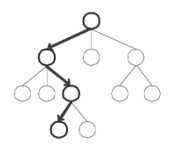
\includegraphics[width=1.0\textwidth]{pics/selection.png}
		
		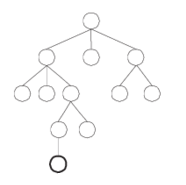
\includegraphics[width=1.0\textwidth]{pics/expansion.png}
		
		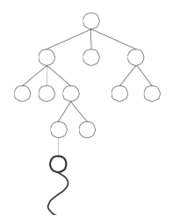
\includegraphics[width=1.0\textwidth]{pics/simulation.png}
		
		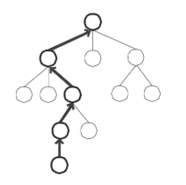
\includegraphics[width=1.0\textwidth]{pics/backpropagation.png}
	\end{minipage}
	
\subsection{Evolutionary Algorithms (EA)}
	
	\begin{tabular}{C{0.1\textwidth}p{0.3\textwidth}p{0.6\textwidth}}
		\toprule
		Symbol & Name &  Description \\
		\midrule
		$i$ & individual/solution & a possible solution for the problem at hand\\
		$P$ & population of individuals & set of possible solutions\\
		$t$ & time-step or generation & \\
		$P_t, P(t)$ & population at time $t$ & \\
		$\mu, N$ & (number of) individuals in $P$ & equal to $\vert P \vert$ \\ 
		$M$ & mating pool & individuals selected for genetic operators\\
		$\lambda$ & (number of) inidividuals in $M$ & set of children\\
		$f_i$ & fitness of individual $i$ & scoring the fitness of an individual based on an objective function\\
		$p_i$ & selection probability of individual $i$ & probability of an individual being selected for the mating pool\\
		\bottomrule
	\end{tabular}
	\vskip3em
	\begin{algorithm}[H]
		\DontPrintSemicolon
		\KwIn{Initial Population $P(t)$}
		$t \leftarrow 0$\;
		\;
		\Repeat{termination condition}{
			Select individuals for genetic operators: $M(t) \leftarrow \textit{selection}(P(t))$\;
			Apply Crossover: $\;\!M'(t) \leftarrow \textit{crossover}(M(t))$\;
			Apply Mutation: $M''(t) \leftarrow \textit{mutation}(M'(t))$\;
			Update $P(t)$: $~\;P(t+1) \leftarrow \textit{reproduction\_scheme}(P(t) \cup M''(t))$\;
			$t \leftarrow t+1$\;
		}
		\KwOut{Final Population $P(t)$}    
		\caption{General Evolutionary Algorithm}
	\end{algorithm}
	

\subsection{Rolling Horizon (RH)}

	\begin{algorithm}[H]
		\DontPrintSemicolon
		\KwIn{current state $s_t$, horizon h}
		\;
		$E \leftarrow$ simulate a random episode starting at $s_t$ till timestep $t+h$\;
		\;
		\Repeat{time is over}{
			$E' \leftarrow$ simulate a random episode starting at $s_t$ till timestep $t+h$\;
			\If{Return of $E' >$ Return of $E$}{
				$E \leftarrow E'$\;
			}
		}
		\;
		\KwOut{First action of E}    
		\caption{Rolling Horizon Random Search}
	\end{algorithm}
	\vskip2em
	\begin{algorithm}[H]
		\DontPrintSemicolon
		\KwIn{current state $s_t$, horizon h}
		\;
		$P \leftarrow$ population of random episodes starting at $s_t$ till timestep $t+h$\;
		\;
		\Repeat{time is over}{
			$M \leftarrow$ select individuals from P for genetic operators \;
			$M' \leftarrow$ apply crossover to $M$\;
			$M'' \leftarrow$ apply mutation to $M'$\;
			$P \leftarrow$ apply reproduction scheme to $(P \cup M'')$\;
		}
		\;
		\KwOut{First action of the episode with the highest return in P}    
		\caption{Rolling Horizon Evolutionary Algorithm (RHEA)}
	\end{algorithm}

\section{Multi Objective Optimization}


\subsection{General Notation}

	\begin{tabular}{C{0.1\textwidth}p{0.3\textwidth}p{0.6\textwidth}}
		\toprule
		Symbol & Name &  Description \\
		\midrule
		$S$ & search space & the space of all possible solutions\\
		$O$ & objective space & $O = \lbrace \vec{f}(x) \in \mathbb{R}^m \vert x \in S \rbrace$\\
		$\vec{f}(x)$ & objective vector & all objective values for individual x \\
		$f_i$ & objective function & assigns an objective value to each solution\\
		$f_i(x)$ & i-th objective value of x& \\
		$r_i$ & rank of solution i & see the lecture for ranking methods \\
		$d_i$ & (crowding) distance of i & specifically used in NSGA-II \\
		$\Omega_i(x)$ & cone domination & cone-dominating version of objective function $f_i$\\
		$C(A, B)$ & convergence metric & compare the convergence between two non-dominated set of points $A$ and $B$\\
		$HV(A)$ & hyper-volume of $A$ & calculate the hyper-volume of a non-dominated set of solutions $A$\\
		$MHV(i)$ & marginal hyper volume of individual $i$ & $MHV(i) = HV(entire~Set) - HV(set~without~i)$\\
		
		\bottomrule
	\end{tabular}

\subsection{NSGA-II Algorithm}

	\begin{algorithm}[H]
		\DontPrintSemicolon
		\KwIn{Individuals of Population $P(t)$ and the Mating Pool $M(t)$}
		Fronts $(F_1, F_2, \cdots) \leftarrow$ non-dominated sorting of $P(t) \cap M(t)$\;
		Set $P(t+1) = \emptyset, \quad i=1, \quad N = P(t)$\;
		\vskip1.0em
		\Repeat{$\vert P(t+1)\vert + \vert F_i\vert \leq N$}{
			$P(t+1) \leftarrow P(t+1)\cap F_i$\;
			$i \leftarrow i+1$\;
		}
		\vskip1.0em
		Sort all individuals in $F_i$ by their crowding distance\;
		$P(t+1) \leftarrow P(t+1)~\cap $ $\lbrace$first $N-\vert P(t+1)\vert$ elements in $F_i\rbrace$\;
		\vskip1.0em
		\KwOut{Next Population $P(t+1)$}    
		\caption{NSGA-II Algorithm}
	\end{algorithm}

\end{document}
